% Lab 2 LaTeX Document
% Version 1.1
\documentclass{article}
\usepackage{listings}
\usepackage[margin=1in]{geometry}
\usepackage{graphicx}
\usepackage{textcomp}
\usepackage[pdftex,
            pdfauthor={Daniel Noyes},
            pdftitle={Laboratory \#2 - Spring 2016 },
            pdfsubject={ECE 368 Digital Design},
            pdfkeywords={Digital Design, VHDL, Nexys 2, Xilinx, ISE},
            pdfproducer={Latex},
            pdfcreator={pdflatex}]{hyperref}

%Remove the number display for each section tag
\makeatletter
\renewcommand\@seccntformat[1]{}
\makeatother

\begin{document}

\begin{center}
\textsc{\huge ECE 368 Digital Design - Spring 2016}\\[1cm]
\textsc{{\LARGE Laboratory \#2: (100pts)}}\\[0.5cm]
\textsc{\Large Lab date: February $5$\textsuperscript{th},2016}\\[0.5cm]
\textsc{\Large Lab Report Due: Friday February $12$\textsuperscript{th},2016}\\[1cm]
\end{center}

\section{Overview and Objectives:}
In this laboratory assignment, you will be using the Xilinx ISE Design tools aimed at the Digilent Nexys 2 development board to become familiar with the VHDL design code entry, verification and simulation. You will be able to understand the principles of I/O systems and learn how to build your own interface with the various I/O's on the board. You will also examine the use of test bench's for design verification and develop and demonstrate a hardware text procedure.

\section{Objectives for this lab:}
\begin{itemize}
  \item An introduction to understand VHDL code
  \item Learn the process of building and flashing on a Nexys 2 dev board
  \item Understand basic input/output (I/O)
  \item Understand debouncing concepts
  \item Understand VHDL operations that will help build a foundation
  \item Learn how to create a test bench to test a device
  \item Able to read and understand RTL diagrams
  \item Able to assemble all the concepts together
\end{itemize}

\section{Lab sections:}
\begin{enumerate}
  \item Introduction with a counter
  \item Applying button debouncing concepts
  \item More in depth with a 7-Segment Display
  \item Learning how to use a test bench with a ALU
  \item Assembling all you learn together into a ALU with input
\end{enumerate}

\newpage
\section{1. Introduction with a counter:}
The counter described in this section of the lab can be used to create a clock divider in upcoming labs. The counter project contains six files, you don't have to worry about the contents of them for now. Right now you will be focusing on how to build this project first and then we will explain how it works.

\subsection{Creating New Project in ISE Design Suite}

You will need the counter project code which can be found \href{https://github.com/reiuiji/ECE368-Lab/tree/master/Lab%202/Counter}{here} or in the class directory.
Now lets start ISE Project Navigator. When you open up Xilinx ISE project navigator, you will be greeted by the welcome screen. You need to create a new project, you can do this either from the welcome screen or \textbf{File -\textgreater new project}.

\begin{figure}[!h]
  \centering
    \fbox{\includegraphics[width=0.5\textwidth]{images/XilinxNewProject.png}}
  \caption{ISE\textsuperscript{\textregistered} Design Suite welcome page}
\end{figure}

\textbf{Steps for creating a new project in ISE:}
\begin{enumerate}
  \item Select \textbf{File -\textgreater new project} to open the New Project Wizard.
  \item Enter a name for the project, for this project is will be \textbf{MealyTest}
  \item Enter a location where the project will be located
  \item Enter a description for the project
  \item Select \textbf{HDL} in the top-level source type
  \item Click next to advance to the project setting page
  \item Enter the parameters for the project: \hfill \\
  Family : \textbf{Spartan3E}\\
  Device : \textbf{XC3S500E}\\
  Package : \textbf{FG320}\\
  Speed  : \textbf{-4}\\
  Systhesis Tool : \textbf{XST (VHDL/Verilog)}\\
  Simulator : \textbf{ISim (VHDL/Verilog)}\\
  Preferred Language : \textbf{VHDL}\\
  Property Specification in Project File : \textbf{Store all values}\\
  Uncheck Manual Compile Order\\
  VHDL Source Analysis Standard : \textbf{VHDL-93}\\
  Uncheck Message Filtering
  \item Double Check the Project Setting with the Setting Figure
\end{enumerate}

\newpage %temporary fix to get the figures align next to the setup

\begin{figure}[!htb]
  \centering
    \fbox{\includegraphics[width=0.6\textwidth]{images/NewProjectWizard1.png}}
  \caption{New Project Wizard Create New Project page}
\end{figure}

\begin{figure}[!htb]
  \centering
    \fbox{\includegraphics[width=0.6\textwidth]{images/NewProjectWizard2.png}}
  \caption{New Project Wizard Project Settings page}
\end{figure}

\subsection{Adding VHDL Source to the Project}
After you have created the project in ISE. You will now need to import the counter source files into the project. This can be done by going to \textbf{Project -\textgreater Add Source}. Select each of the six files in the Counter folder. After you imported all the files needed you will be presented with a clock\_toplevel file as depicted in the next figure.

\begin{figure}[!htb]
  \centering
    \fbox{\includegraphics[width=0.5\textwidth]{images/XilinxCounterTopLevel.png}}
  \caption{Clock\_toplevel project design}
\end{figure}

\subsection{Building the counter project}
Now since you have a fully setup project. we are now going to build it. When you click on the "clock\_toplevel" it will give you multiple options on the bottom on design tab. For building the project, you must run the "Generate Programming File". This can take a few minutes for ISE to process the VHDL files and create a programming file. During this process is where you will encounter various warnings and errors that may occur while building the project.

\begin{figure}[!htb]
  \centering
    \fbox{\includegraphics[width=0.5\textwidth]{images/XilinxCounterCreateProgramFile.png}}
  \caption{Clock\_toplevel generate program file}
\end{figure}

\subsection{Building issue on a s3e500 board}
While building the counter project, you may encounter an error while mapping the pins on a \textbf{s3e500} board. This can be resolved by changing the led pins in the user constraint file (UCF) file with the ones commented.

\begin{figure}[!htb]
  \centering
    \fbox{\includegraphics[width=0.5\textwidth]{images/CounterMapError.png}}
  \caption{Counter pin mapping error}
\end{figure}

\begin{figure}[!htb]
  \centering
    \fbox{\includegraphics[width=0.5\textwidth]{images/CounterLeducf.png}}
  \caption{Counter User Constraints File - Led}
\end{figure}

\subsection{Flashing the counter project onto the board}
After build the project file you will see a green check mark appear on the "Generate Programming File". This means the project bit file was successfully created. Now it is the time to flash the Nexys 2 FPGA. In order to flash to the Nexys 2, you need to open up ISE iMPACT which can be found in \textbf{Tools -\textgreater iMPACT}.

\begin{figure}[!htb]
  \centering
    \fbox{\includegraphics[width=0.5\textwidth]{images/XilinxImpactLocation.png}}
  \caption{Xilinx iMPACT Location}
\end{figure}

\textbf{Steps to Flash Nexyx 2 with ISE iMPACT}
\begin{enumerate}
  \item Click on \textbf{Boundary Scan} under iMPACT Flows\
  \item Click on \textbf{Initialize Chain} on the tool bar or \textbf{File -\textgreater Initialize Chain} or Ctrl+i.
  \item Wait until it ducceeded on the initialize chain
  \item Click \textbf{Yes} on "Auto Assign Configuration Files".
  \item Select the recently generated bit file in you projects folder
  \item Click \textbf{No} on "Attach SPI or BPI PROM".
  \item On the assign new configuration file select \textbf{Cancel All}.
  \item Click \textbf{OK} on "Device Programming Properties".
  \item Click the \textbf{xc3s500e} chip.
  \item Double click \textbf{Program} under the iMPACT Processes
  \item Wait a few seconds and it will say "Program Succeeded"
  \item Check the Nexys 2 Dev board and if the led are incrementing you now have successfully flashed the Nexys 2.
\end{enumerate}

\subsection{Testing the Nexys 2 Counter}
After you have successfully flashed the Nexys 2. Go play with the Counter and see what switch and button will affect the counter. There are three things you will need to look for on the Board. A reset, add/subtract mode, and change speed of the counter.

\subsection{Counter Layout}
As you might have played around with the device. You noticed that there were three inputs to this counter. The counter is comprised of a few entities, a clock, mux, counter, and a toplevel which binds them all together. You can see the register-transfer level(RTL) in the next figure which gives a block diagram of the project. You can generate you own RTL under \textbf{Design -\textgreater Synthesize - XST -\textgreater View RTL Schematic}

\begin{figure}[!htb]
  \centering
    \fbox{\includegraphics[width=0.5\textwidth]{images/XilinxInitRTL.png}}
  \caption{View RTL Schematic Location}
\end{figure}

\begin{figure}[!htb]
  \centering
    \fbox{\includegraphics[width=0.7\textwidth]{images/CounterRTL.png}}
  \caption{RTL Schematic for the counter}
\end{figure}

\subsection{Breakdown of the Counter}
While looking at the RTL schematic for the counter. You can see two clocks, each with a different name of "clk2Hz" and "clk4Hz". Both are design to toggle after a certain number of cycles, for this one the input to each clock is 50 MHz. Both clock lines will then go through a mux 2 to 1 with a select switch to choose which clock to output. The output of the mux will then go into the clock input of the counter. The counter will add or subtract one from its current count signal. The counter toplevel connects all the components together and the \textbf{counter\_topleve.ucf} will till the toplevel ports to the pins of the FPGA. Look at each file in the project and study how they work.

\subsection{Counter Questions}
While going through each segment you will be asked a few questions. These question will ask you about various parts of the lab besides these questions you will also need to demonstrate your work and knowledge to the TA or Professor. Don't forget to write down your answers and put them in your lab report.

\begin{enumerate}
  \item Demonstrate a working counter. \hfill \\
  Reset the counter value.\\
  Change the counter speed.\\
  Change the counter to subtract instead of adding to the count.
  \item Double the clock rate in the clk4Hz file. What does it do?
  \item What action of the clock causes the counter to add or subtract(Rising Action? or Falling Action?).
  \item What do you think could be different in this section of the lab?
\end{enumerate}

\newpage

\section{2. Applying button debouncing concepts:}
On the Nexys 2 board, there are four mechanical push buttons. These push buttons can be very noisy when you click them. With this in mine, you will need to debounce the push button signal. In this section of the lab you will be learning the concepts of debouncing a signal and how to implement it in your design.

\subsection{Concepts of debouncing a signal}
There are a variety of methods to debounce a signal. The method you will learn uses three flip flops, a xor gate, counter, and a bit compare. The input signal will go through one flip flop and then through another flip flop and will update it state based on the clock line. This will allow us to have two states of the signal. Each state will then go though an XOR gate to monitor the change in state. When there are two different states the xor will output a \textbf{1} to reset the counter. The counter will increment when no change occurs and the most significant bit will be used to update the last flip flop state. The last flip flop will output the debounced signal.

\begin{figure}[!htb]
  \centering
    \fbox{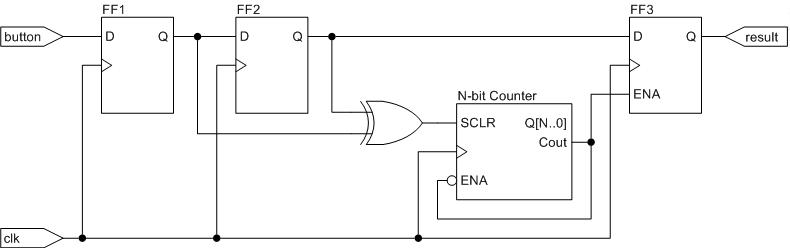
\includegraphics[width=0.7\textwidth]{images/debounce_schematic-from-eewiki.JPG}}
  \caption{Debouncing circuit example(\href{http://eewiki.net/x/FgBM}{Source : eewiki})}
\end{figure}

\subsection{Applying the concepts into VHDL}
With learning the concepts of debouncing a signal. Next we need to apply the concepts into VHDL. First you will be needing signals to maintain the values of the first two flip flops, the XOR output and a location for the counter value. You will need to create a process routine to monitor the clock state. In the process, the flip flops will update their state when there is a \textbf{CLK'event} and with a value of \textbf{1}. This can be translated into a rising action on the clock line. Next you will need to check the flip flop states and reset the counter if both flip flops have different states. The output will happen if the most significant bit will turn \textbf{1}. It is recommend reviewing the debounce.vhd source and get a understanding of what is happening.

\subsection{Building and Flashing the button debouncer project}
Now is the time to build the button debouncer. First create a new project just like in the counter section. Add the source in the Button folder, there will be three files. Build, and flash it on the Nexys 2 dev board(refer to counter). Don't forget to check the VHDL code and see what is happening.

\subsection{Button Debouncing Questions}

\begin{enumerate}
  \item Demonstrate to the TA or professor the button controller.
  \item Why would you incorporate a enable in the button controller?
\end{enumerate}

\newpage

\section{3. More in depth with a 7-Segment Display:}
In this section, you will be learning how a 7-segment display can be incorporated in VHDL. While observing the Nexys 2 dev board, you will notice that there are four 7-segment displays. These displays can be very useful to use as a debug device since there can be 4 bytes of data displayed.

\subsection{Reviewing 7-Segment Display}
Just refresher each 7-segment display is tied to a common cathode while one anode per display. The cathodes are a ground sink while the anode supply the power. For the display you do not want to have the number flicker. So the display should oscillate around 60Hz. Since there are four displays you need to alternate between them. This will give us 240Hz for alternating between each number without flickering.

\subsection{Applying the concepts into VHDL}
In order to apply this in VHDL, you need to break down the 7-segment driver into reasonable chunks. First you will need a clock divider that will change a 50Mhz clock signal into 240Hz. Next you will need a 7-segment decoder, this can be done in a select statement in VHDL. The Last major part is the display driver to cycle between the 7-segment display and output the correct number. Look at the SevenSeg.vhd file to get a grasp of the concept. The top level connects the SevenSeg out to the board and helps provide values for the 7-segment display.

\subsection{Building and Flashing the 7-segment Display project}
Create a new project and add the source in the "SevenSegment" folder. Build the 7-segment display and flash it to the Nexys. Test the Seven Segment display by flipping the dip switches to control the first two displays.

\subsection{7-Segment Display Questions}

\begin{enumerate}
  \item Adjust the VHDL code I/O to make the 7-seg display "FACE"
  \item Demonstrate to the TA or professor the 7-seg display
  \item What is the clock speed in the 7-segment display driver and why?
\end{enumerate}

\begin{figure}[!htb]
  \centering
    \fbox{\includegraphics[width=0.5\textwidth]{images/7segFACE.png}}
  \caption{7-segment Display output FACE}
\end{figure}

\newpage

\section{4. Learning how to use a test bench with a ALU:}
In this section of the lab, you will be getting familiar with simulating VHDL in ISE. You are presented a complete source of an ALU. A ALU is a Arithmetic device which will output specific values based on operating codes(opcodes). For the ALU you will have two 8 bit input values(A,B) and a opcode. The output will have the result of the operation plus a condition code register.
\subsection{Concepts of a ALU}
In this Lab you will be using an 8-bit ALU. The ALU is a collection of operations. These operations can be add, subtract, AND, OR, Shift and much more. For the ALU you can see what operations it performs based on the opcodes in the table below.

\begin{table}[!htb]
  \begin{center}
    \begin{tabular}{|l|l|l|l|}
       \hline
       OPCODE & operation & procedure & CCR\\
       \hline 
       0000 & ADDITION & RA \textless = RA + RB & NZVC \\
       0001 & SUBTRACTION & RA \textless = RA - RB & NZVC \\
       0010 & AND & RA \textless = RA \& RB & NZVC \\
       0011 & OR & RA \textless = RA \textbar \enspace RB & NZVC \\
       0100 & COMPARE & RA \textless = 0, NZ change & NZ \\
       0101 & ADD Immediate & RA \textless = RA + IMMED & NZVC \\
       0110 & AND Immediate & RA \textless = RA \& IMMED & NZVC \\
       0111 & SHIFT LEFT & RA \textless = RA$<<$IMMED & VC \\
       1000 & SHIFT RIGHT & RA \textless = RA$>>$IMMED  & \\
       1001 & LOAD WORD & RA \textless = ALU\_MEM  & \\
       1010 & STORE WORD & ALU\_MEM \textless = RA & \\
       \hline
    \end{tabular}
  \end{center}
  \caption{ALU OPCODE}
\end{table}

\subsection{Setting up a ALU in VHDL}
Create a new project or use a existing and remove the files. Add all the source files in the ALU folder to the project. In this project you will be using the simulation utility in Xilinx. In order to run a simulation, you will need to create a Behavioral vhd file. This file will simulate the inputs to a VHDL design you are implementing. This will be able to aid in testing your code for and prone errors that may arise during your testing of the code.

\subsection{Testing the ALU by simulation}
In order to start simulation you must switch you view from Implementation to Simulation, this can be done by \textbf{Design -\textgreater View -\textgreater Simulation}. When you in simulation mode, select \textbf{ALU\_tb\_vhd}. Under the design tab you will see ISim Simulation and two operations. \textbf{Behavioral Check Syntax} and \textbf{Simulate Behavioral Model}. Run the Simulate Behavioral Model, there will be a graph popping up with the simulation results from the test bench file.

\begin{figure}[!htb]
  \centering
    \fbox{\includegraphics[width=0.5\textwidth]{images/XilinxSelectSimulation.png}}
  \caption{Select Simulation Mode in ISE}
\end{figure}

\begin{figure}[!htb]
  \centering
    \fbox{\includegraphics[width=0.5\textwidth]{images/XilinxStartSimulation.png}}
  \caption{Start Simulation in ISE}
\end{figure}

\newpage
\subsection{ALU test bench Questions}
\begin{enumerate}
  \item Take a screen shot of the simulation from 50ns - 300ns
  \item Change CCR value at line 110 from \textbf{1010} to \textbf{0000}. Rerun the simulation, what do you notice in the console and why does it happen?
\end{enumerate}

\newpage

\section{5. Assembling all you learn together into a ALU with input:}
With each section you learned various concepts and was given code to run. Now it is your turn to create some VHDL code. In the previous sections you learned how to interface with the Nexys board Dip switches, Led's, mechanical buttons, and the seven segment display. You also learned about a ALU. For this section you will be combining them together and creating a user input ALU. The method of input and output is all up to you.

\subsection{Jumping into VHDL}
Since this will be your first time coding VHDL for the project. You will have to devise a method for your ALU to interface with. First you need to create a block diagram of each device connected together. After that give more in depth design in a RTL. Build your design in VHDL with a reference of the top\_level designs in the other sections of the lab.

\subsection{Building, Flashing and testing a user input ALU project}
This part will take you the most time to accomplish out of all the sections. You will have to debug you code and see how it runs on the Nexys 2 dev board. The building and flashing will always be the same methods in any lab. You will also be needing to create a Acceptance Test Plan(ATP) to validate that your project is working.

\subsection{Final Questions}
\begin{enumerate}
  \item Demonstrate to the TA or professor the user input ALU.
  \item What was the biggest challenge you overcame?
  \item If you would rebuild this, how you change it?
  \item What is your confidence level in VHDL and explain why.
  \item Any ideas to improve the Lab?
\end{enumerate}

\newpage

\section{Lab 2 Grade}

\begin{table}[!htb]
  \begin{center}
    \begin{tabular}[width=0.8\textwidth]{|l|l|c|l|}
       \hline
       Section & Description & Value & Score\\
       \hline 
       \multicolumn{2}{|l}{\textbf{Section 1}}  & -10- &\\
       \hline
       1.1. Counter Demo & Demonstrate Counter to TA, Prof & 5 &\\
       1.2. Counter Questions & Answer Questions about the Counter & 5 &\\
       \hline
       \multicolumn{2}{|l}{\textbf{Section 2}}  & -10- &\\
       \hline
       2.1. Button Demo & Demonstrate Button to TA, Prof & 5 &\\
       2.2. Button Questions & Answer Questions about the Button Debouncer & 5 &\\
       \hline
       \multicolumn{2}{|l}{\textbf{Section 3}}  & -10- &\\
       \hline
       3.1. 7-Seg Demo & Demonstrate 7-Seg with display of \textbf{FACE} & 5 &\\
       3.2. 7-Seg Questions & Answer Questions about the 7-Segment Display & 5 &\\
       \hline
       \multicolumn{2}{|l}{\textbf{Section 4}}  & -10- &\\
       \hline
       4.1. Screen shot of simulation &  Screen shot of the simulation & 5 &\\
       4.2. ALU Sim Questions & Answer Questions about the ALU Simulation & 5 &\\
       \hline
       \multicolumn{2}{|l}{\textbf{Section 5}}  & -10- &\\
       \hline
       5.1. ALU User Input Demo & Demonstrate ALU to TA, Prof & 5 &\\
       5.2. ALU User Input Questions & Answer Questions about the ALU & 5 &\\
       \hline
       \multicolumn{2}{|l}{\textbf{Lab Report}}  & -50- &\\
       \hline
       \hline
       \multicolumn{2}{|l}{Total} & \multicolumn{1}{c|}{100} &\\
       \hline
    \end{tabular}
  \end{center}
  \caption{Lab Grade Breakdown Table}
\end{table}

\end{document}
